\documentclass{beamer}
\mode<presentation>
\usetheme{CambridgeUS}
\usepackage[russian]{babel}
\usepackage[utf8]{inputenc}
\usepackage[T2A]{fontenc}
\usepackage{sansmathaccent}

\usepackage{verbatim}
\usepackage{alltt}

\pdfmapfile{+sansmathaccent.map}
\title[Основы алгоритмизации]{Основы алгоритмизации}
\author{Наумов Д.А., доц. каф. КТ}
\date[11.02.2019] {Программирование и алгоритмические языки, 2019}

\begin{document}

%ТИТУЛЬНЫЙ СЛАЙД
\begin{frame}
  \titlepage
\end{frame}
  
%СОДЕРЖАНИЕ ЛЕКЦИИ
\begin{frame}
  \frametitle{Содержание лекции}
  \tableofcontents  
\end{frame}

\section{Этапы решения задач}
\begin{frame}{Этапы решения задач на ЭВМ}
Решение любой задачи на ЭВМ состоит из нескольких этапов, среди которых основными являются следующие:
\begin{enumerate}
\item постановка задачи;
\item формализация (математическая постановка задачи);
\item выбор метода решения;
\item разработка алгоритма;
\item составление программы;
\item отладка программы;
\item вычисление и обработка результатов.
\end{enumerate}
Последовательное выполнение перечисленных этапов составляет полный цикл разработки.
\end{frame} 

\begin{frame}
\begin{block}{При постановке задачи}
первостепенное внимание должно уделяться выяснению конечной цели и выработке общего подхода к исследуемой проблеме. Правильно сформулировать задачу иногда не менее сложно, чем ее решить.
\end{block}
\begin{block}{Формализация}
сводится к построению математической модели рассматриваемого явления, когда в результате анализа задачи:
\end{block}
\begin{itemize}
\item определяются объем и специфика исходных данных;
\item вводится система условных обозначений;
\item устанавливается принадлежность решаемой задачи к одному из известных классов задач;
\item выбирается соответствующий математический аппарат;
\end{itemize}
\end{frame}

\begin{frame}
\begin{block}{Выбор метода решения}
необходим после того, как определена математическая формулировка задачи.
\end{block}
\begin{itemize}
\item применение любого метода приводит к построению ряда формул и к формулировке правил, определяющих связи между этими формулами;
\item все это разбивается на отдельные действия так, чтобы вычислительный процесс мог быть выполнен машиной;
\end{itemize}
\end{frame}

\begin{frame}
\begin{block}{Разработка алгоритма}
данный этап заключается в разложении вычислительного процесса на возможные составные части, установлении порядка их следования, описании содержания каждой такой части в той или иной форме.
\end{block}
В процессе разработки алгоритм проходит несколько этапов детализации. 
\begin{itemize}
\item первоначально составляется укрупненная схема алгоритма, в которой отражаются наиболее важные и существенные  связи между исследуемыми процессами. 
\item на последующих этапах раскрываются выделенные на предыдущих этапах части вычислительного процесса.
\end{itemize}
\end{frame}

\section{Основы алгоритмизации}
\begin{frame}
\begin{block}{Алгоритм}
однозначно определенная на некотором языке конечная последовательность предписаний (инструкций, команд), задающая порядок исполнения элементарных операций для систематического решения задачи.
\end{block}
Семь параметров, характеризующих алгоритм:
\begin{enumerate}
\item Совокупность возможных исходных данных.
\item Совокупность возможных результатов.
\item Совокупность возможных промежуточных результатов.
\item Правило начала процесса обработки данных.
\item Правило непосредственной обработки.
\item Правило окончания обработки.
\item Правило извлечения результата. 
\end{enumerate}
Алгоритм должен обладать свойствами: массовость, результативность. 
\end{frame}

%средства записи алгоритмов
\begin{frame}
Средства записи алгоритмов
\begin{enumerate}
\item текстуальная форма записи;
\item схемы алгоритмов;
\item диаграммы Нэсси-Шнейдермана;
\item диаграммы Дейкстры;
\item псевдокод;
\item запись в форме программы на языке программирования;
\item ДРАКОН-схемы;
\item Р-схемы
\end{enumerate}
\end{frame}

\begin{frame}
\begin{block}{Текстуальная форма записи алгоритма}
\begin{figure}[h]
\centering
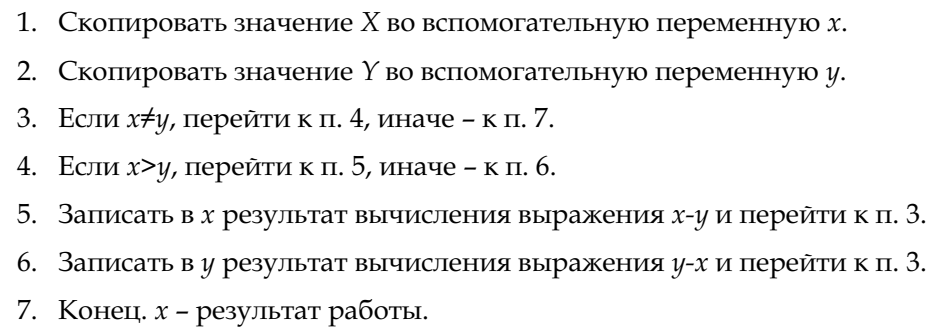
\includegraphics[scale=0.45]{images/lec01-pic01.png}
\end{figure}
\end{block}
\begin{itemize}
\item + наименее формализованная
\item - не обеспечивается наглядность решения
\end{itemize}
\end{frame}

\begin{frame}
\begin{block}{Блок-схема алгоритма}
\begin{figure}[h]
\centering
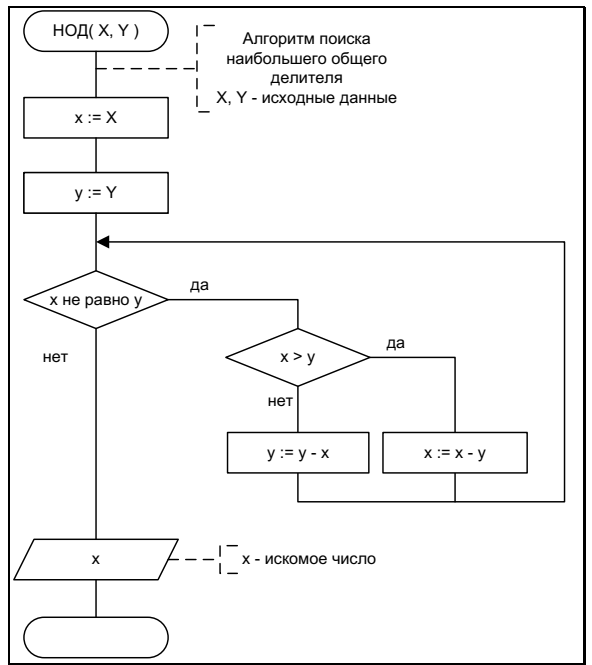
\includegraphics[scale=0.35]{images/lec01-pic02.png}
\end{figure}
\end{block}
\begin{itemize}
\item + регулируются стандартом ISO 5807-85 и российским [ГОСТ 19.701-90]
\item - обеспечивают наглядность только для простых алгоритмов
\end{itemize}
\end{frame}

\begin{frame}
\begin{block}{Диаграммы Нэсси-Шнейдермана}
\begin{figure}[h]
\centering
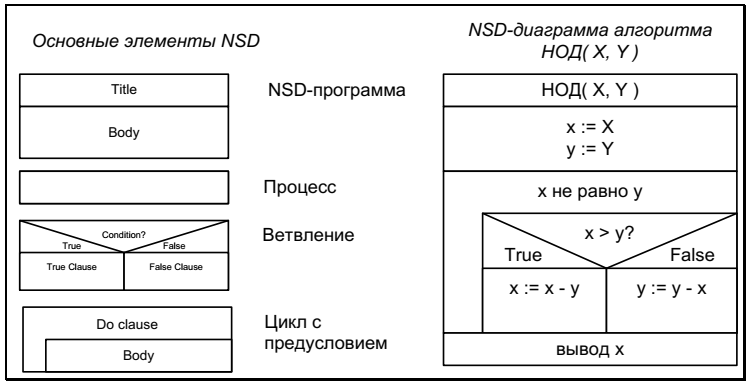
\includegraphics[scale=0.35]{images/lec01-pic03.png}
\end{figure}
\end{block}
\begin{itemize}
\item + менее запутанные, чем текст и блок-схемы
\item + методически удобны при обсуждении областей видимости программных объектов
\item - для сложных программ либо внешний прямоугольник будет очень большим, либо внутренние элементы – слишком маленькими
\end{itemize}
\end{frame}

\begin{frame}
\begin{block}{Диаграммы Дейкстры}
\begin{figure}[h]
\centering
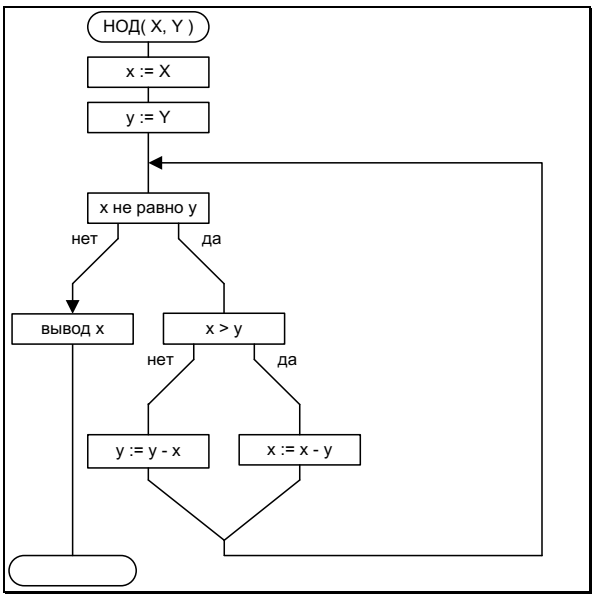
\includegraphics[scale=0.35]{images/lec01-pic04.png}
\end{figure}
\end{block}
\begin{itemize}
\item + "более ограниченная" топология, чем текст и блок-схемы
\item - не был востребованы разработчиками стандартов на схемы алгоритмов и программ
\end{itemize}
\end{frame}

\begin{frame}
\begin{block}{Псевдокод}
\begin{figure}[h]
\centering
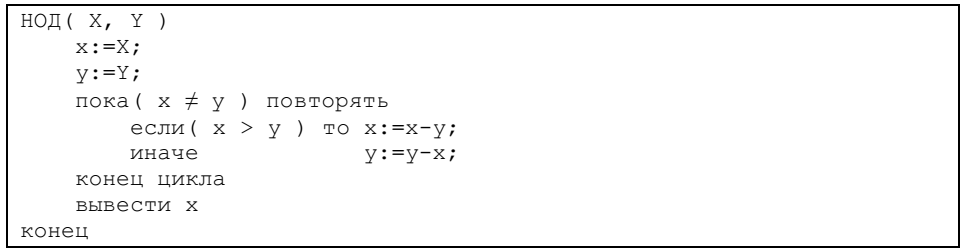
\includegraphics[scale=0.35]{images/lec01-pic05.png}
\end{figure}
\end{block}
\begin{itemize}
\item + эффективная форма текстуальной записи алгоритма, абстрагированная от конкретного языка
\item + используется, когда программисты хотят отложить окончательную запись решения на более позднее время
\end{itemize}
\end{frame}

\begin{frame}
\begin{block}{Запись на языке C}
\begin{figure}[h]
\centering
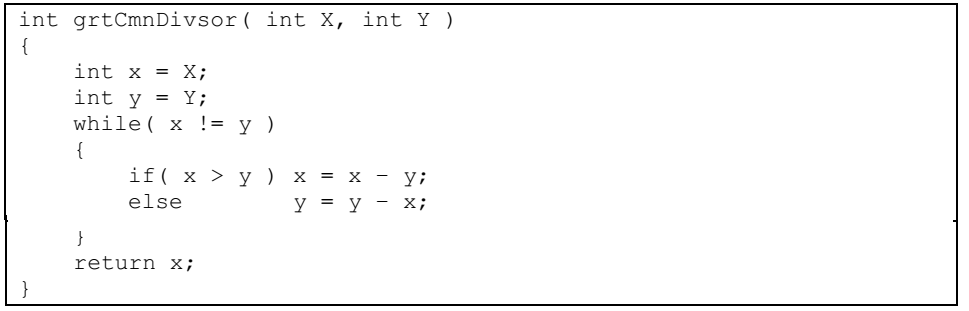
\includegraphics[scale=0.35]{images/lec01-pic06.png}
\end{figure}
\end{block}
\begin{block}{Запись на языке Pascal}
\begin{figure}[h]
\centering
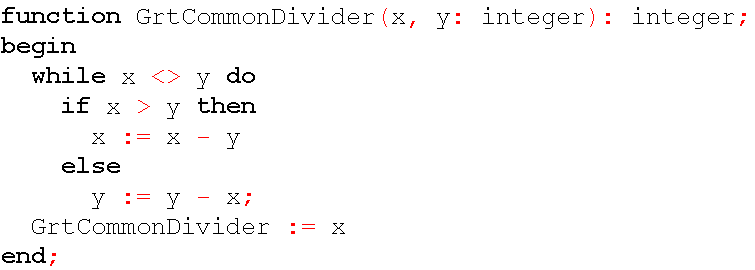
\includegraphics[scale=0.35]{images/lec01-pic07.png}
\end{figure}
\end{block}
\end{frame}

\begin{frame}
\begin{block}{Запись на визуальном языке ДРАКОН}
\begin{figure}[h]
\centering
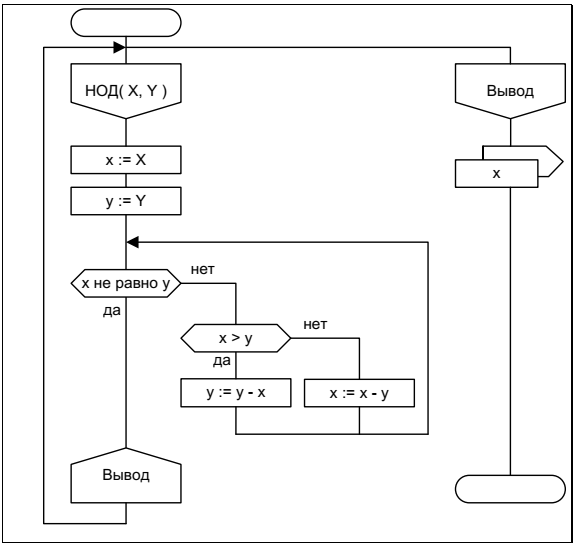
\includegraphics[scale=0.4]{images/lec01-pic08.png}
\end{figure}
\end{block}
Построен на основе визуального языка ДРАКОН и на основе шампур-метода
как абстрактной визуальной модели программы.
\end{frame}

\begin{frame}
\begin{block}{Р-схемы}
\begin{figure}[h]
\centering
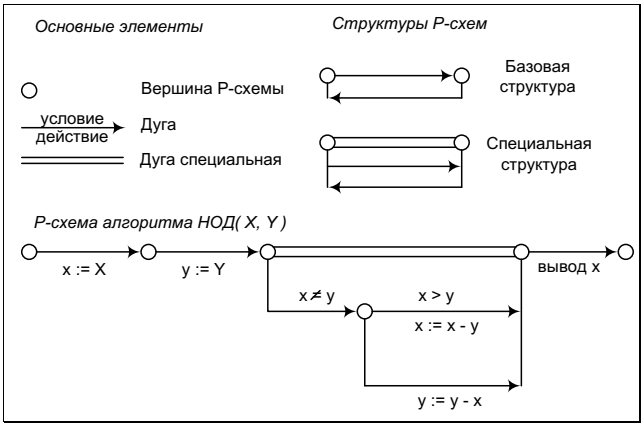
\includegraphics[scale=0.4]{images/lec01-pic09.png}
\end{figure}
\end{block}
Р-схемы являются центральным элементом визуального ядра Р-технологии, разработанной в институте кибернетики Академии наук Украины.
\end{frame}

\section{Основные элементы алгоритмических языков программирования}
%алфавит
\begin{frame}
\begin{block}{Алфавит}
набор символов (литер), используемых для записи программ.
\end{block}
Из литер конструируются лексемы (tokens) – относительно обособленные элементы синтаксических конструкций языка. Наиболее распространены пять основных категорий лексем:
\begin{itemize}
\item идентификаторы – для записи символических имен программных объектов;
\item ключевые слова, которые, вообще говоря, являются специальным классом идентификаторов – для записи инструкций языка;
\item литералы: целочисленные, с плавающей точкой, символьные, строковые – для записи констант;
\item знаки операций (арифметических, логических, операций отношения и др.) – для записи элементарных действий над данными;
\item знаки пунктуации – однолитерные лексемы, используемые для
структурирования и организации программного кода.
\end{itemize}
\end{frame}

\begin{frame}
\begin{block}{Алфавит языка C++}
\begin{figure}[h]
\centering
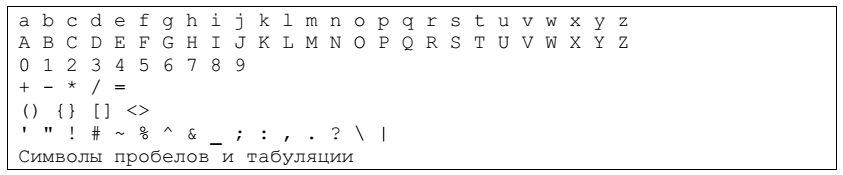
\includegraphics[scale=0.4]{images/lec01-pic10.png}
\end{figure}
\end{block}
\begin{block}{Алфавит языка Pascal}
\begin{figure}[h]
\centering
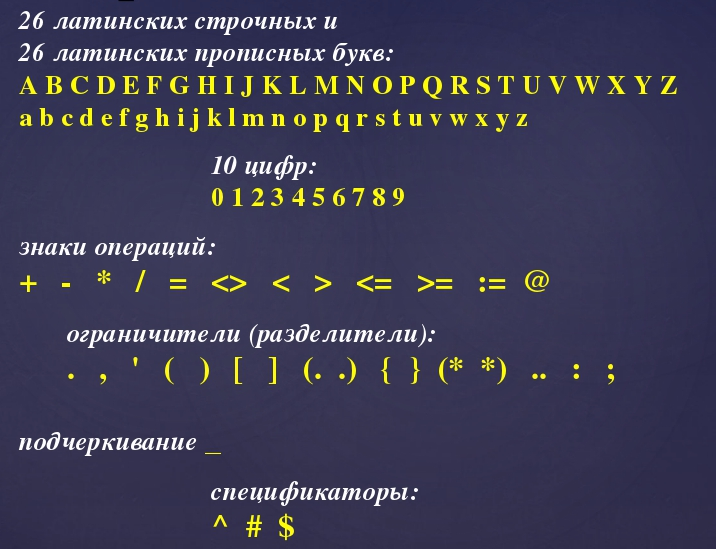
\includegraphics[scale=0.3]{images/lec01-pic11.png}
\end{figure}
\end{block}
\end{frame}

%синтаксис и семантика
\begin{frame}
\begin{block}{Трансляция}
перевод программы на компилируемом языке высокого уровня в программу на машинных кодах
\end{block}
При трансляции cмысл программы не должен измениться, должна измениться только форма ее представления, так как правила составления предложений языка строго
регламентированы синтаксисом и семантикой. 
\begin{block}{Синтаксис}
правила построения языка и его конструкций.
\end{block}
\begin{block}{Семантика}
строго определенный смысл каждой конструкции языка.
\end{block}
\end{frame}

\begin{frame}
\begin{block}{Синтаксически-ориентированная трансляция}
вычисление единственно возможного смысла программного кода на
основании анализа синтаксиса.
\begin{figure}[h]
\centering
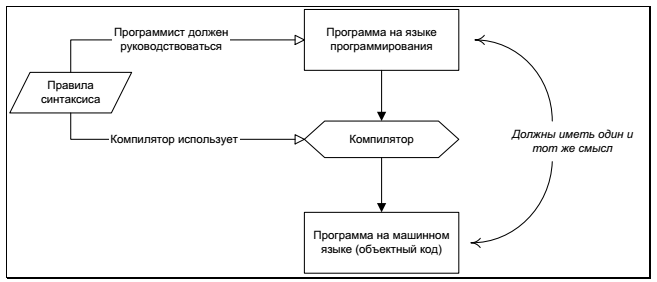
\includegraphics[scale=0.6]{images/lec01-pic12.png}
\end{figure}
\end{block}
\end{frame}

\begin{frame}
\begin{block}{Синтаксис и семантика}
\begin{figure}[h]
\centering
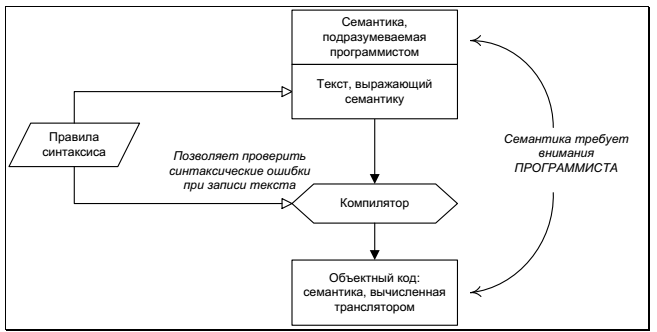
\includegraphics[scale=0.6]{images/lec01-pic13.png}
\end{figure}
\end{block}
\end{frame}

%формы Бэкуса-Науэра
\begin{frame}
\begin{block}{Описание синтаксиса в форме правил Бэкуса-Наура}
\begin{figure}[h]
\centering
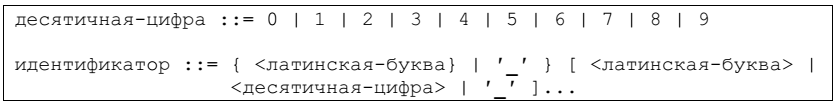
\includegraphics[scale=0.5]{images/lec01-pic14.png}
\end{figure}
\end{block}
\end{frame}

\begin{frame}
\begin{block}{Синтаксические диаграммы Н. Вирта}
\begin{figure}[h]
\centering
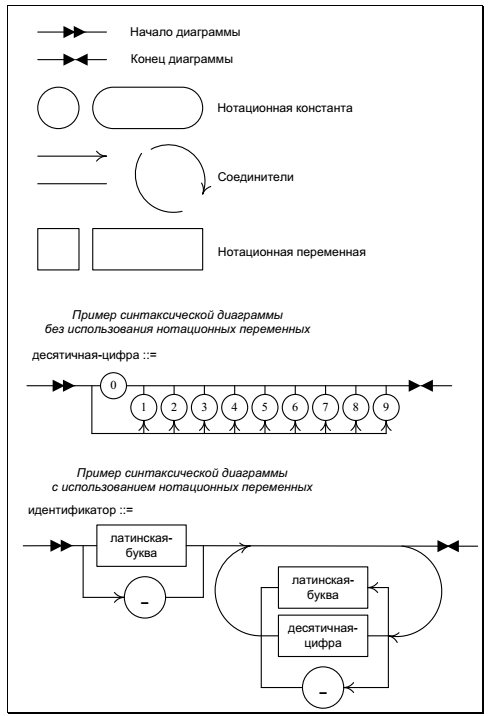
\includegraphics[scale=0.35]{images/lec01-pic15.png}
\end{figure}
\end{block}
\end{frame}

%идентификаторы
\begin{frame}
\begin{block}{Идентификатор}
одна из основных синтаксических конструкций, используемых в программах. 
\end{block}
\begin{itemize}
\item любое имя, используемое в программе, должно быть идентификатором;
\item идентификатор может состоять из одного или более символов (латинских букв, цифр, символов подчеркивания);
\item первым символом должна быть латинская буква или знак подчеркивания;
\item максимальная длина идентификатора зависит от компилятора.
\end{itemize}
\begin{block}{Регситр символов}
\begin{itemize}
\item не важен для языка Pascal;
\item важен для языка C/C++.
\end{itemize}
\end{block}
\end{frame}

\begin{frame}
\begin{itemize}
\item ряд идентификаторов явно зарезервирован для нужд языка. Это –
ключевые (служебные) слова языка;
\item идентификаторы, начинающиеся с двойного подчеркивания, или с подчеркивания, вслед за которым следует прописная буква, считаются зарезервированными для использования системой (С++). 
\item в некоторых средах разработки существуют свои стандарты,
которым рекомендуется следовать, если предполагается совместное
использование программного кода коллективами разработчиков.
\end{itemize}
\end{frame}

%ключевые слова
\begin{frame}
\begin{block}{Ключевые слова}
идентификаторы, имеющие предопределенный смысл в языке.
\end{block}
Ключевые слова языка С
\begin{figure}[h]
\centering
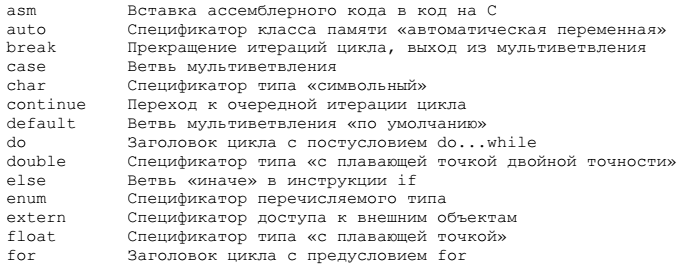
\includegraphics[scale=0.6]{images/lec01-pic16.png}
\end{figure}
\end{frame}

\begin{frame}
Ключевые слова языка Pascal
\begin{figure}[h]
\centering
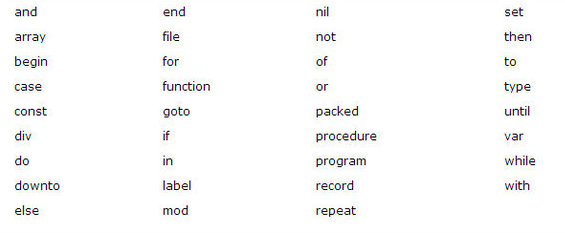
\includegraphics[scale=0.6]{images/lec01-pic17.png}
\end{figure}
\end{frame}

%запись текстов программ
\begin{frame}
Правила записи текстов программ могут быть:
\begin{itemize}
\item жестко зафиксированы (взаимное расположение конструкций языка жестко регламентировано);
\item полуфиксированными (в ассемблерных языках, Python);
\item свободным (Pascal, C/C++).
\end{itemize}
При свободной записи текстов программ:
\begin{itemize}
\item синтаксические конструкции могут начинаться с любой позиции строки текста программы;
\item одна инструкция может располагаться в нескольких строках программы
\item несколько инструкций могут располагаться в одной строке
\item между отдельными лексемами может быть помещен один
или более пробелов или других символов пробельной группы (табуляции,
символы перевода строки)
\item поскольку символ конца строки считается символом-разделителем,
один идентификатор не может располагаться на нескольких строчках
\end{itemize}
\end{frame}

\begin{frame}
Рекомендованные правила оформления исходного кода:
\begin{itemize}
\item вертикальное форматирование: действия, составляющие один
логический блок, комментарии, сопровождающие текст, символы,
ограничивающие обособленные блоки (например, фигурные
скобки в языке C++, пары ключевых слов begin, end в языке Pascal)
записываются друг под другом с выравниванием по левому краю.
\item Горизонтальное форматирование: при оформлении перехода к
вложенному логическому блоку (в ветвлениях и циклах)
используются отступы, или табуляции.
\item Оставляются пустые строчки между обособленными логическими
фрагментами, определениями функций, структурами данных и т.д.
\item Текст организуется таким образом, что в
отдельной строке помещается одна высокоуровневая инструкция,
за естественным исключением тех случаев, когда группа
инструкций образует единое целое в синтаксическом или в
математическом смысле.
\end{itemize}
\end{frame}

%комментарии
\begin{frame}
\begin{block}{Комментарии}
инструмент сопровождения программного кода. 
\end{block}
Комментарии языка С/С++
\begin{figure}[h]
\centering
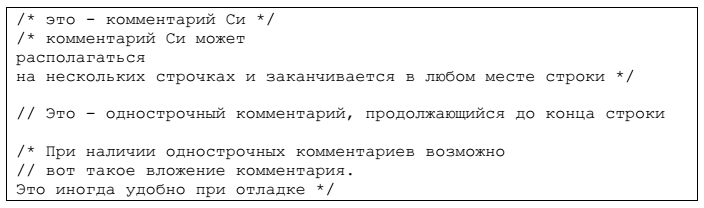
\includegraphics[scale=0.5]{images/lec01-pic18.png}
\end{figure}
Комментарии языка Pascal
\begin{figure}[h]
\centering
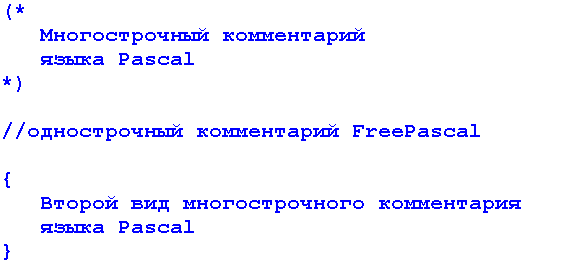
\includegraphics[scale=0.4]{images/lec01-pic19.png}
\end{figure}
\end{frame}

\begin{frame}
Виды комментариев с точки зрения их назначения:
\begin{itemize}
\item \textbf{заголовочные, или титульные, комментарии} - комментарии в
начале файла (модуля), содержащие, в частности, информацию об
имени файла (и, возможно, расшифровку этого имени).
\item \textbf{выделяющие, или предваряющие, комментарии} -
размещаются перед относительно обособленными фрагментами
текста, служат промежуточными заголовками к группам данных
или действий или объясняют назначение отдельных подпрограмм.
\item \textbf{сопровождающие, или поясняющие, комментарии} - обычно
располагаются справа от основного текста и предназначены не
только для пояснения отдельных моментов, но и просто облегчают
читателю (в том числе и самому проектировщику) ориентирование
в тексте.
\item \textbf{констатирующие комментарии} - подводят итог некоторого
фрагмента, указывают на состояние программы или каких-либо
данных по достижении этой точки программы.
\end{itemize}
\end{frame}

\end{document}
